%  LaTeX support: latex@mdpi.com 
%DIF LATEXDIFF DIFFERENCE FILE
%DIF DEL D:/CINVESTAV/Doctorado/Cuatrimestre/7/Dr Deni/TrafficModel/tmp.old.tex                 Tue Nov  3 19:40:02 2020
%DIF ADD D:/CINVESTAV/Doctorado/Cuatrimestre/7/Dr Deni/TrafficModel/Vehicle Traffic Model.tex   Tue Nov  3 19:38:43 2020
%  In case you need support, please attach all files that are necessary for compiling as well as the log file, and specify the details of your LaTeX setup (which operating system and LaTeX version / tools you are using).

%=================================================================
\documentclass[sensors,article,submit,moreauthors,pdftex]{Definitions/mdpi} 





\usepackage{amsmath}
\usepackage[center]{subfigure} %para las subfiguras
\usepackage{multirow}
\DeclareMathOperator*{\argmax}{arg\,max}
\DeclareMathOperator*{\argmin}{arg\,min}
\newcommand{\mathvec}[1]{\boldsymbol{\mathbf{\MakeLowercase{#1}}}}
\newcommand{\mathmat}[1]{\boldsymbol{\mathbf{\MakeUppercase{#1}}}}
\newcommand{\mathten}[1]{\boldsymbol{\mathbf{\mathcal{\MakeUppercase{#1}}}}}




% If you would like to post an early version of this manuscript as a preprint, you may use preprint as the journal and change 'submit' to 'accept'. The document class line would be, e.g., \documentclass[preprints,article,accept,moreauthors,pdftex]{mdpi}. This is especially recommended for submission to arXiv, where line numbers should be removed before posting. For preprints.org, the editorial staff will make this change immediately prior to posting.

%--------------------
% Class Options:
%--------------------
%----------
% journal
%----------
% Choose between the following MDPI journals:
% acoustics, actuators, addictions, admsci, aerospace, agriculture, agriengineering, agronomy, algorithms, animals, antibiotics, antibodies, antioxidants, applsci, arts, asc, asi, atmosphere, atoms, axioms, batteries, bdcc, behavsci , beverages, bioengineering, biology, biomedicines, biomimetics, biomolecules, biosensors, brainsci , buildings, cancers, carbon , catalysts, cells, ceramics, challenges, chemengineering, chemistry, chemosensors, children, cleantechnol, climate, clockssleep, cmd, coatings, colloids, computation, computers, condensedmatter, cosmetics, cryptography, crystals, dairy, data, dentistry, designs , diagnostics, diseases, diversity, drones, econometrics, economies, education, ejihpe, electrochem, electronics, energies, entropy, environments, epigenomes, est, fermentation, fibers, fire, fishes, fluids, foods, forecasting, forests, fractalfract, futureinternet, futurephys, galaxies, games, gastrointestdisord, gels, genealogy, genes, geohazards, geosciences, geriatrics, hazardousmatters, healthcare, heritage, highthroughput, horticulturae, humanities, hydrology, ijerph, ijfs, ijgi, ijms, ijns, ijtpp, informatics, information, infrastructures, inorganics, insects, instruments, inventions, iot, j, jcdd, jcm, jcp, jcs, jdb, jfb, jfmk, jimaging, jintelligence, jlpea, jmmp, jmse, jnt, jof, joitmc, jpm, jrfm, jsan, land, languages, laws, life, literature, logistics, lubricants, machines, magnetochemistry, make, marinedrugs, materials, mathematics, mca, medicina, medicines, medsci, membranes, metabolites, metals, microarrays, micromachines, microorganisms, minerals, modelling, molbank, molecules, mps, mti, nanomaterials, ncrna, neuroglia, nitrogen, notspecified, nutrients, ohbm, optics, particles, pathogens, pharmaceuticals, pharmaceutics, pharmacy, philosophies, photonics, physics, plants, plasma, polymers, polysaccharides, preprints , proceedings, processes, proteomes, psych, publications, quantumrep, quaternary, qubs, reactions, recycling, religions, remotesensing, reports, resources, risks, robotics, safety, sci, scipharm, sensors, separations, sexes, signals, sinusitis, smartcities, sna, societies, socsci, soilsystems, sports, standards, stats, surfaces, surgeries, sustainability, symmetry, systems, technologies, test, toxics, toxins, tropicalmed, universe, urbansci, vaccines, vehicles, vetsci, vibration, viruses, vision, water, wem, wevj

%---------
% article
%---------
% The default type of manuscript is "article", but can be replaced by: 
% abstract, addendum, article, benchmark, book, bookreview, briefreport, casereport, changes, comment, commentary, communication, conceptpaper, conferenceproceedings, correction, conferencereport, expressionofconcern, extendedabstract, meetingreport, creative, datadescriptor, discussion, editorial, essay, erratum, hypothesis, interestingimages, letter, meetingreport, newbookreceived, obituary, opinion, projectreport, reply, retraction, review, perspective, protocol, shortnote, supfile, technicalnote, viewpoint
% supfile = supplementary materials

%----------
% submit
%----------
% The class option "submit" will be changed to "accept" by the Editorial Office when the paper is accepted. This will only make changes to the frontpage (e.g., the logo of the journal will get visible), the headings, and the copyright information. Also, line numbering will be removed. Journal info and pagination for accepted papers will also be assigned by the Editorial Office.

%------------------
% moreauthors
%------------------
% If there is only one author the class option oneauthor should be used. Otherwise use the class option moreauthors.

%---------
% pdftex
%---------
% The option pdftex is for use with pdfLaTeX. If eps figures are used, remove the option pdftex and use LaTeX and dvi2pdf.

%=================================================================
\firstpage{1} 
\makeatletter 
\setcounter{page}{\@firstpage} 
\makeatother
\pubvolume{xx}
\issuenum{1}
\articlenumber{5}
\pubyear{2019}
\copyrightyear{2019}
%\externaleditor{Academic Editor: name}
\history{Received: date; Accepted: date; Published: date}
%\updates{yes} % If there is an update available, un-comment this line

%% MDPI internal command: uncomment if new journal that already uses continuous page numbers 
%\continuouspages{yes}

%------------------------------------------------------------------
% The following line should be uncommented if the LaTeX file is uploaded to arXiv.org
%\pdfoutput=1

%=================================================================
% Add packages and commands here. The following packages are loaded in our class file: fontenc, calc, indentfirst, fancyhdr, graphicx, lastpage, ifthen, lineno, float, amsmath, setspace, enumitem, mathpazo, booktabs, titlesec, etoolbox, amsthm, hyphenat, natbib, hyperref, footmisc, geometry, caption, url, mdframed, tabto, soul, multirow, microtype, tikz


%=================================================================
%% Please use the following mathematics environments: Theorem, Lemma, Corollary, Proposition, Characterization, Property, Problem, Example, ExamplesandDefinitions, Hypothesis, Remark, Definition, Notation, Assumption
%% For proofs, please use the proof environment (the amsthm package is loaded by the MDPI class).

%=================================================================
% Full title of the paper (Capitalized)
\Title{Tensor Modeling and Analysis for Vehicle Traffic}

% Author Orchid ID: enter ID or remove command
\newcommand{\orcidauthorA}{0000-0000-000-000X} % Add \orcidA{} behind the author's name
%\newcommand{\orcidauthorB}{0000-0000-000-000X} % Add \orcidB{} behind the author's name

% Authors, for the paper (add full first names)
\Author{Hermosillo-Reynoso Fernando $^{1,\ddagger}$*, Torres-Roman Deni $^{1,\ddagger}$}

% Authors, for metadata in PDF
\AuthorNames{Fernando Hermosillo-Reynoso, Deni Torres-Roman}

% Affiliations / Addresses (Add [1] after \address if there is only one affiliation.)
\address{%
	$^{1}$ \quad CINVESTAV IPN Department of Electrical Engineering and Computer Sciences, Telecommunications Section, Guadalajara, Jalisco, Mexico; fhermosillo@gdl.cinvestav.mx; dtorres@gdl.cinvestav.mx}
%$^{1}$ \quad Affiliation 1; e-mail@e-mail.com\\
%$^{2}$ \quad Affiliation 2; e-mail@e-mail.com}

% Contact information of the corresponding author
\corres{Correspondence: fhermosillo@gdl.cinvestav.mx; Tel.: +52-331-631-3095}

% Current address and/or shared authorship
%\firstnote{Current address: Affiliation 3} 
\secondnote{These authors contributed equally to this work.}
% The commands \thirdnote{} till \eighthnote{} are available for further notes

%\simplesumm{} % Simple summary

%\conference{} % An extended version of a conference paper


% Abstract (Do not insert blank lines, i.e. \\) 
\abstract{A single paragraph of about 200 words maximum. For research articles, abstracts should give a pertinent overview of the work. We strongly encourage authors to use the following style of structured abstracts, but without headings: (1) Background: Place the question addressed in a broad context and highlight the purpose of the study; (2) Methods: Describe briefly the main methods or treatments applied; (3) Results: Summarize the article's main findings; and (4) Conclusion: Indicate the main conclusions or interpretations. The abstract should be an objective representation of the article, it must not contain results which are not presented and substantiated in the main text and should not exaggerate the main conclusions.}

% Keywords
\keyword{keyword 1; keyword 2; keyword 3 (list three to ten pertinent keywords specific to the article, yet reasonably common within the subject discipline.)}

% The fields PACS, MSC, and JEL may be left empty or commented out if not applicable
%\PACS{J0101}
%\MSC{}
%\JEL{}

%%%%%%%%%%%%%%%%%%%%%%%%%%%%%%%%%%%%%%%%%%
% Only for the journal Diversity
%\LSID{\url{http://}}

%%%%%%%%%%%%%%%%%%%%%%%%%%%%%%%%%%%%%%%%%%
% Only for the journal Applied Sciences:
%\featuredapplication{Authors are encouraged to provide a concise description of the specific application or a potential application of the work. This section is not mandatory.}
%%%%%%%%%%%%%%%%%%%%%%%%%%%%%%%%%%%%%%%%%%

%%%%%%%%%%%%%%%%%%%%%%%%%%%%%%%%%%%%%%%%%%
% Only for the journal Data:
%\dataset{DOI number or link to the deposited data set in cases where the data set is published or set to be published separately. If the data set is submitted and will be published as a supplement to this paper in the journal Data, this field will be filled by the editors of the journal. In this case, please make sure to submit the data set as a supplement when entering your manuscript into our manuscript editorial system.}

%\datasetlicense{license under which the data set is made available (CC0, CC-BY, CC-BY-SA, CC-BY-NC, etc.)}

%%%%%%%%%%%%%%%%%%%%%%%%%%%%%%%%%%%%%%%%%%
% Only for the journal Toxins
%\keycontribution{The breakthroughs or highlights of the manuscript. Authors can write one or two sentences to describe the most important part of the paper.}

%\setcounter{secnumdepth}{4}
%%%%%%%%%%%%%%%%%%%%%%%%%%%%%%%%%%%%%%%%%%
%DIF PREAMBLE EXTENSION ADDED BY LATEXDIFF
%DIF UNDERLINE PREAMBLE %DIF PREAMBLE
\RequirePackage[normalem]{ulem} %DIF PREAMBLE
\RequirePackage{color}\definecolor{RED}{rgb}{1,0,0}\definecolor{BLUE}{rgb}{0,0,1} %DIF PREAMBLE
\providecommand{\DIFadd}[1]{{\protect\color{blue}\uwave{#1}}} %DIF PREAMBLE
\providecommand{\DIFdel}[1]{{\protect\color{red}\sout{#1}}}                      %DIF PREAMBLE
%DIF SAFE PREAMBLE %DIF PREAMBLE
\providecommand{\DIFaddbegin}{} %DIF PREAMBLE
\providecommand{\DIFaddend}{} %DIF PREAMBLE
\providecommand{\DIFdelbegin}{} %DIF PREAMBLE
\providecommand{\DIFdelend}{} %DIF PREAMBLE
\providecommand{\DIFmodbegin}{} %DIF PREAMBLE
\providecommand{\DIFmodend}{} %DIF PREAMBLE
%DIF FLOATSAFE PREAMBLE %DIF PREAMBLE
\providecommand{\DIFaddFL}[1]{\DIFadd{#1}} %DIF PREAMBLE
\providecommand{\DIFdelFL}[1]{\DIFdel{#1}} %DIF PREAMBLE
\providecommand{\DIFaddbeginFL}{} %DIF PREAMBLE
\providecommand{\DIFaddendFL}{} %DIF PREAMBLE
\providecommand{\DIFdelbeginFL}{} %DIF PREAMBLE
\providecommand{\DIFdelendFL}{} %DIF PREAMBLE
%DIF LISTINGS PREAMBLE %DIF PREAMBLE
\RequirePackage{listings} %DIF PREAMBLE
\RequirePackage{color} %DIF PREAMBLE
\lstdefinelanguage{DIFcode}{ %DIF PREAMBLE
%DIF DIFCODE_UNDERLINE %DIF PREAMBLE
  moredelim=[il][\color{red}\sout]{\%DIF\ <\ }, %DIF PREAMBLE
  moredelim=[il][\color{blue}\uwave]{\%DIF\ >\ } %DIF PREAMBLE
} %DIF PREAMBLE
\lstdefinestyle{DIFverbatimstyle}{ %DIF PREAMBLE
	language=DIFcode, %DIF PREAMBLE
	basicstyle=\ttfamily, %DIF PREAMBLE
	columns=fullflexible, %DIF PREAMBLE
	keepspaces=true %DIF PREAMBLE
} %DIF PREAMBLE
\lstnewenvironment{DIFverbatim}{\lstset{style=DIFverbatimstyle}}{} %DIF PREAMBLE
\lstnewenvironment{DIFverbatim*}{\lstset{style=DIFverbatimstyle,showspaces=true}}{} %DIF PREAMBLE
%DIF END PREAMBLE EXTENSION ADDED BY LATEXDIFF

\begin{document}
%%%%%%%%%%%%%%%%%%%%%%%%%%%%%%%%%%%%%%%%%%

%%%%%%%%%%%%%%%%%%%%%%%%%%%%%%%%%%%%%%%%%%
%\setcounter{section}{-1} %% Remove this when starting to work on the template.
%\section{How to Use this Template}
%The template details the sections that can be used in a manuscript. Note that the order and names of article sections may differ from the requirements of the journal (e.g., the positioning of the Materials and Methods section). Please check the instructions for authors page of the journal to verify the correct order and names. For any questions, please contact the editorial office of the journal or support@mdpi.com. For LaTeX related questions please contact latex@mdpi.com.
%The order of the section titles is: Introduction, Materials and Methods, Results, Discussion, Conclusions for these journals: aerospace,algorithms,antibodies,antioxidants,atmosphere,axioms,biomedicines,carbon,crystals,designs,diagnostics,environments,fermentation,fluids,forests,fractalfract,informatics,information,inventions,jfmk,jrfm,lubricants,neonatalscreening,neuroglia,particles,pharmaceutics,polymers,processes,technologies,viruses,vision

\section{Introduction}
%The introduction should briefly place the study in a broad context and highlight why it is important. It should define the purpose of the work and its significance. The current state of the research field should be reviewed carefully and key publications cited. Please highlight controversial and diverging hypotheses when necessary. Finally, briefly mention the main aim of the work and highlight the principal conclusions. As far as possible, please keep the introduction comprehensible to scientists outside your particular field of research. Citing a journal paper \cite{ref-journal}. And now citing a book reference \cite{ref-book}. Please use the command \citep{ref-journal} for the following MDPI journals, which use author-date citation: Administrative Sciences, Arts, Econometrics, Economies, Genealogy, Humanities, IJFS, JRFM, Languages, Laws, Religions, Risks, Social Sciences.
Content
\begin{enumerate}[leftmargin=*,labelsep=4.9mm]
\item	Related work.
\item	Contribution.
\item	Content.
\end{enumerate}


%%%%%%%%%%%%%%%%%%%%%%%%%%%%%%%%%%%%%%%%%%
\section{Tensor Algebra}
\label{sec:tensoralg}
\begin{table}[H]
\caption{Tensor Algebra Notation Summary.}
\centering
%% \tablesize{} %% You can specify the fontsize here, e.g., \tablesize{\footnotesize}. If commented out \small will be used.
\begin{tabular}{ll}
\midrule
$\mathten{X}, \mathmat{X}, \mathvec{x}, x$		& Tensor, matrix, vector scalar.\\
$\mathten{X} \in \mathbb{R}^{I_1 \times \cdots \times I_N}$		& A ${I_1 \times \cdots \times I_N}$ tensor.\\
$ord(\mathten{X})$ & The order of a tensor.\\
$x_{i_1 \cdots i_N}$ & The $({i_1 \cdots i_N})$ entry of an $N^{th}$-order tensor.\\
$\mathmat{X}^{(n)}$ & The $n^{th}$ matrix element from a sequence of matrices.\\
$\mathmat{X}_{(n)}$ & The n-mode matricization of a tensor.\\
$\boldsymbol{\otimes}$ & Outer product of two vectors.\\
$\boldsymbol{\otimes}_{kron}$ & Kronecker product of two matrices.\\
$\bigodot$	& Khatri Rao product of two matrices.\\
$\langle \mathten{X}, \mathten{Y} \rangle$ & Inner product of two tensors.\\
$\mathten{Y} = \mathten{X} \times_n \mathmat{U}$ & The n-mode product of a tensor $\mathten{X}$ times a matrix $\mathmat{U}$ along the $n$ dimension.\\
$[\![\boldsymbol{\lambda}/\mathten{G},\mathmat{U}^{(1)},\cdots,\mathmat{U}^{(N)}]\!]$ & Kruskal notation of tensor decomposition models.\\
$rank_{D}(\mathten{X})=R$ & Tensor decomposition/CP rank.\\
$rank_{tc}(\mathten{X})=(R_1,\cdots, R_N)$ & Tensor multilinear/Tucker rank, where $R_n = rank(\mathmat{X}_{(n)})$.\\
$rank_k(\mathten{X})$ & Tensor Kruskal-rank\\
\textemdash\textemdash	 & \textemdash\textemdash\textemdash\textemdash\textemdash\textemdash\textemdash\textemdash\textemdash\\
$\mathten{X} * \mathten{Y}$ & t-product of two tensors.\\
$\mathten{X} *_{\Phi} \mathten{Y}$ & $\Phi$-product of two tensors.\\
\textemdash\textemdash	 & \textemdash\textemdash\textemdash\textemdash\textemdash\textemdash\textemdash\textemdash\textemdash\\
$\mathcal{H}(\cdot)$/$\mathcal{H}^{-1}(\cdot)$ & Hankelization direct/inverse transformation.\\
$\mathcal{L}(\cdot)$/$\mathcal{L}^{-1}(\cdot)$ & L{\"o}wnerization direct/inverse transformation.\\
\textemdash\textemdash	 & \textemdash\textemdash\textemdash\textemdash\textemdash\textemdash\textemdash\textemdash\textemdash\\
$\mathten{V}_\tau$ & Video of duration $\tau$, represented as a tensor.\\
$\mathten{B}$ & Background tensor.\\
$\mathten{F}$ & Foreground tensor.\\
$\mathten{T}^{(N)}$ & Vehicle traffic feature tensor with $N$ embedded models.\\
\bottomrule
\end{tabular}
\end{table}

% n-mode product of a tensor $\mathten{X}\in\mathbb{R}^{I_1 \times \cdots \times I_N}$ times a matrix $\mathmat{U} \in \mathbb{R}^{J \times I_n}$ along the n-dimension resulting in a tensor $\mathten{Y} \in \mathbb{R}^{I_1 \times \cdots \times I_{n-1} \times J \times I_{n+1} \times \cdots \times I_N}$.

\begin{enumerate}[leftmargin=*,labelsep=4.9mm]
	\item	Notation.
	\item	Basic tensor concepts.
	\item 	Operators on tensors.
	\item 	Tensorization definition and methods.
	\item	Tensor decompositions (E.G.)
	\begin{enumerate}[leftmargin=*,labelsep=4.9mm]
		\item	CANDECOM/PARAFAC Decomposition
		\item	Tucker Decomposition
		\item	Tensor Robust PCA
	\end{enumerate}
\end{enumerate}
%%%%%%%%%%%%%%%%%%%%%%%%%%%%%%%%%%%%%%%%%%



%%%%%%%%%%%%%%%%%%%%%%%%%%%%%%%%%%%%%%%%%%
\section{Problem Statement and Mathematical Definition}

Current traffic surveillance systems employ different data models on each stage, so there is no such unified model which allows to capture relationships among all stages. Multidimensional models, have proven to be very powerful for explicitly representing and extracting multidimensional structures in several fields, including signal processing [], machine learning [],  and telecommunications [], to name just a few. Unfortunately, despite its high potential in several fields, multidimensional models have not yet been exploited for the vehicle traffic modeling.



\subsection{Problem Statement}
Given a traffic surveillance video $\mathten{V}_\tau$ of duration $\tau$, we seek to formulate a complete and flexible tensor modeling for the supervision of moving vehicles traffic, which allows us to link various data models involved during the analysis of the moving vehicle behavior and its intrinsic interactions among multiple tasks such as: vehicle detection, counting, tracking, occlusion management and classification, as well as to speed up or facilitate data transformation by using certain mathematical operations of tensor algebra.



\subsection{Mathematical Definition}
The problem raised above can be understood as a multidimensional modeling of moving vehicles which we called Vehicle Traffic Feature (VTF) tensor model, in such a way that each data model employed, can be represented as a mode or dimension, i.e., $\mathten{T} \in \mathbb{R}^{Model\:1 \times Model\:2 \times \cdots \times Model\:N}$. Moreover, other representations could be also derived by either fixing certain dimensions or applying some multidimensional operators on it, in order to study the behavior of moving vehicles at specific modes.


%%%%%%%%%%%%%%%%%%%%%%%%%%%%%%%%%%%%%%%%%%



%%%%%%%%%%%%%%%%%%%%%%%%%%%%%%%%%%%%%%%%%%
\section{Tensor-based Vehicle Traffic Modeling}
Traditional vehicle traffic models treat data as a one-dimensional features vector [], to later be used to capture the internal correlation of historical data. However, vehicle traffic data is multi-mode by experiments, e.g., features mode, time mode, vehicle class mode, occlusion mode, among others, therefore, the current models turn out to be inadequate to capture these multidimensional interactions. The proposal of a multidimensional model will preserve the multi-mode nature of data, while the use of tensor methods such as decompositions, will help to better capture correlations among all modes.

\subsection{Traffic Surveillance Video Modeling}

Given a traffic surveillance video modeled as a four-order tensor $\mathten{V}_\tau \in \mathbb{R}^{W\times H \times D \times Time}$ of width and height $W \times H$ resolution with a duration of $\tau$ seconds, and where each pixel is mapped in some color-space in $\mathbb{R}^D$, such as binary, grayscale, and RGB. Then, we will assume that there exist some tensor decomposition model such that Equation \ref{eq:tsvmodel} holds (see Figure \ref{fig:tsvmodel}):

\begin{equation}
\mathten{V}_\tau = \mathten{B} + \mathten{F}
\label{eq:tsvmodel}
\end{equation}

where $\mathten{B} \in \mathbb{R}^{W\times H \times D \times Time}$ represents the background, which can be modeled as a low-rank tensor that capture the lowest frequency component of the video, while $\mathten{F} \in \mathbb{R}^{W\times H \times D \times Time}$ represents the foreground modeled as a sparse tensor containing motion information of the video. Note that in Figure \ref{fig:tsvmodel} exists another tensor denoted by $\mathten{F}_m \in \mathbb{R}^{W\times H \times Time}$, which is the mask of $\mathten{F}$ that is obtained by applying some binary operations on it.

\begin{figure}[H]
\centering
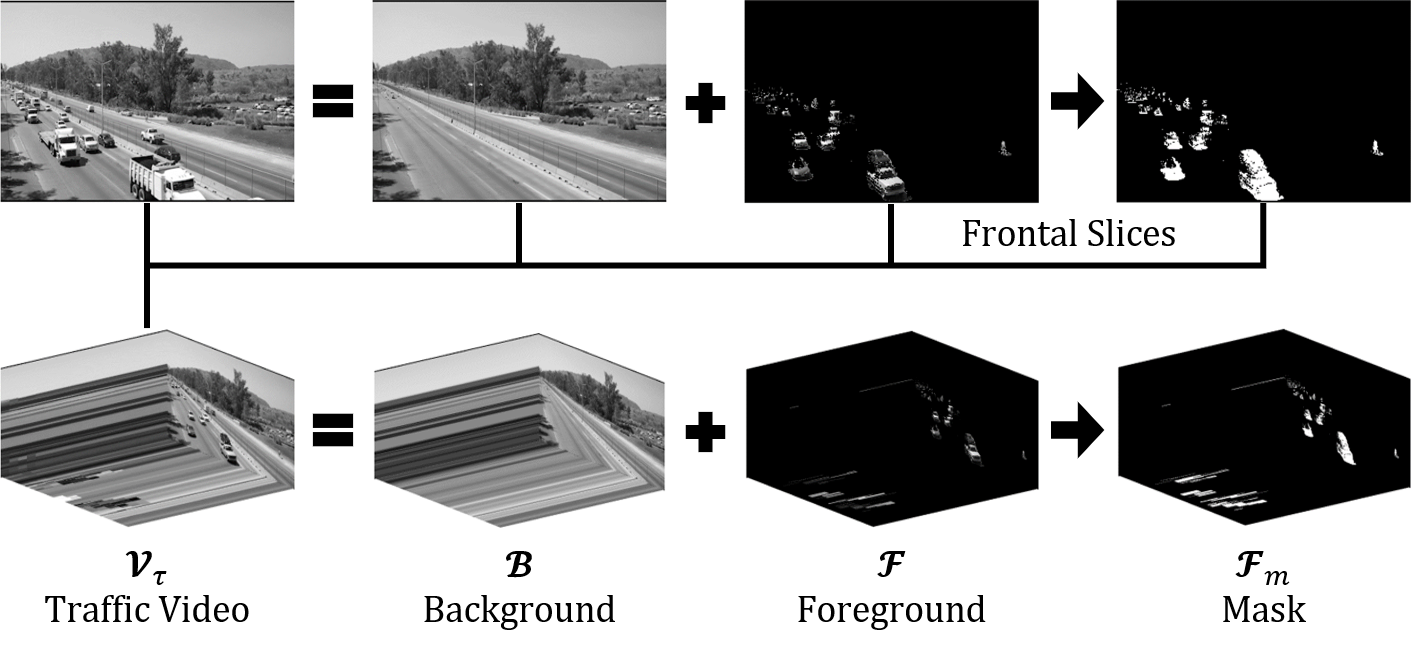
\includegraphics[width=14 cm]{images/traffic-model.png}
\caption{Illustration of the traffic surveillance video decomposition model.}
\label{fig:tsvmodel}
\end{figure}

For this model, there exist some methods and algorithms that successfully decompose a traffic surveillance video into the background and foreground components such as the Gaussian Mixture Model [X], Robust Principal Component Analysis [X], and the pixel-entropy [X] (see [X] for an extensive review on this decomposition). In this work, we will use the Tensor Robust Principal Component Analysis or t-RPCA in short, originally proposed by Lu, C., et. al., [X] to achieve such decomposition.

\subsection{Moving Vehicle Traffic Tensor Modeling}

From the foreground tensor $\mathten{F}$, information about moving vehicles can be extracted such as their trajectory, geometry, kinematic or color information, which can be used later at a particular task of a VTS system. However, due to the high-volume of data and multimodality induced by multi-task VTS systems, a one-mode representation results to be not enough to exploit interactions among tasks.

To tackle the shortcomings of one-mode models, we proposed to arrange and group vehicle information as a high-order structure $\mathten{T}^{(N)} \in \mathbb{R}^{I_1 \times \cdots \times I_N}$, here called Vehicle Traffic Feature (VTF) tensor, to model the vehicle behavior of a feature model over multiple tasks. Even though there is a vast set of features which can be extracted from $\mathten{F}$, here we will focus on the geometric feature model.


%, where the superscript $(N)$ denotes the number of data models embedded on it, in other words its order $N=ord(\mathten{T}^{(N)})$. Therefore, whenever we want to include a new data model, the order of the VTF tensor will increase by one. This will enable us to have a flexible model in the face of new data models.

%In order to construct $\mathten{T}^{(N)}$, during a certain amount of time and for each detected vehicle on the road, we will record a set of geometric features modeled as vectors in $\mathbb{R}^n$, such as area, while assuming that within the observation time, $M$ vehicles will be detected and tracked. Based on these principles, we arrange the recorded data associated to the $i$th vehicle into a matrix $\mathmat{T}_i \in \mathbb{R}^{Geometric\,Features \times Time}$, such that each $\mathmat{T}_i$ will be stacked to form a new tensor $\mathten{T}^{(3)} \in \mathbb{R}^{Vehicle \times Geometric\,Features \times Time}$ or the third-order VTF tensor which will model the behavior of the vehicle geometric features over time.

In order to construct $\mathten{T}^{(N)}$, for each detected vehicle on the road, we will record a set of geometric features modeled as vectors in $\mathbb{R}^n$ during a certain amount of time, while assuming that within the observation time, $M$ vehicles will be detected and tracked. Based on these principles, we arrange the historical data of the $i$th vehicle into a matrix $\mathmat{T}_i \in \mathbb{R}^{F \times t}$, where $F$ denotes the number of features, and $t$ the time. Then, each $\mathmat{T}_i$ will be stacked along the third-dimension, such that the VTF tensor $\mathten{T}^{(3)}$ of Equation \ref{eq:vtf3model} will be formed to model the temporal behavior of the vehicles geometric features.
%Timestamp

\begin{equation}
\mathten{T}^{(3)} \in \mathbb{R}^{Vehicle \times Geometric\,Features \times Time}
\label{eq:vtf3model}
\end{equation}

Following the above ideas, additional modes can also be added for a more generalized modeling of the vehicle geometric features. Specifically, in addition to the three modes of vehicles, geometric features and time, we also include the classification and occlusion modes using the VTF tensor model $\mathten{T}^{(5)}$ as Equation \ref{eq:vtf5model} shows to extend our analysis to multiple stages. In this setting, the classification mode will categorize vehicles according to their sizes (e.g., small, midsize, and large), while the occlusion mode, the type of occlusion [] (e.g., non-occluded, lateral, and queue occlusions).

\begin{equation}
\mathten{T}^{(5)} \in \mathbb{R}^{Vehicles \times Geometric\,Features \times Time \times Class \times Occlusion}
\label{eq:vtf5model}
\end{equation}

\subsubsection{Multilinear Transformations over the Vehicle Traffic Feature Tensor}
For any problem which involves \DIFdelbegin \DIFdel{the use of }\DIFdelend tensor structures, TD allow us to  exploit the intrinsic \DIFdelbegin \DIFdel{high-order }\DIFdelend \DIFaddbegin \DIFadd{multidimensional }\DIFaddend structure of data, therefore, choosing an appropriate representation of data is a key \DIFdelbegin \DIFdel{component }\DIFdelend \DIFaddbegin \DIFadd{ingredient }\DIFaddend to improve any decomposition model. Multilinear \DIFdelbegin \DIFdel{transformations, which aim to express a multidimensional vector space $V_1 \times \cdots \times V_n$ as their multilinear combination by applying some mapping function of several variables that is linear separately in each variable (see Equation \ref{eq:mltransform}) , allow to find other data representations }\DIFdelend \DIFaddbegin \DIFadd{Transformations (MLT) }[] \DIFadd{allow us to represent high-order tensors in different ways by imposing some structured representation on data }\DIFaddend that could be more suitable for a particular TD. \DIFdelbegin %DIFDELCMD < 

%DIFDELCMD < %%%
\begin{displaymath}
\DIFdel{f : V_1 \times \cdots \times V_n \rightarrow W
%DIFDELCMD < \label{eq:mltransform}%%%
}\end{displaymath}%DIFAUXCMD
%DIFDELCMD < 

%DIFDELCMD < %%%
\DIFdel{Similar to linear transformations, multilinear transformations also provide us different properties or structures }%DIFDELCMD < [] %%%
\DIFdel{that can be exploited according to the problem faced, hence the use of a particular transformation must be application dependent. }\DIFdelend Here, we \DIFdelbegin \DIFdel{will seek }\DIFdelend \DIFaddbegin \DIFadd{are seeking }\DIFaddend for those functions which provide a higher-order representation of data while inducing well-known intrinsic structures\DIFdelbegin \DIFdel{. The first desired property will be needed for both preserving linear mixtures of the source space and avoids to introduce non-separable terms }%DIFDELCMD < []%%%
\DIFdel{, while the second property will allow us to enjoy useful properties to be exploited in TD. For that purpose, we employed two deterministic multilinear transformations called }\DIFdelend \DIFaddbegin \DIFadd{, where from all possible known MLT that hold the above, we focus on the deterministic }\DIFaddend Hankelization and L{\"o}wnerization (see Definition \ref{def:hankeltrans} and \ref{def:loewnertrans}), which \DIFdelbegin \DIFdel{map the source space into a higher-order structure that have approximately an intrinsic low multilinear-rank }%DIFDELCMD < [%%%
\DIFdel{x}%DIFDELCMD < ]%%%
\DIFdel{. On the other hand, these transformations enjoy some useful properties for data modeling, for example, Hankel structures are known for representing exponential polynomials }%DIFDELCMD < []%%%
\DIFdel{, while }\DIFdelend \DIFaddbegin \DIFadd{transform the input space into an structured higher-order Hankel or }\DIFaddend L{\"o}wner \DIFdelbegin \DIFdel{structures show a very close relationship with rational functions }\DIFdelend \DIFaddbegin \DIFadd{tensor that intrinsically enforcing an approximately low multilinear-rank }\DIFaddend [\DIFaddbegin \DIFadd{x}\DIFaddend ]\DIFdelbegin \DIFdel{, so that they can be used to model and approximate a wide variety of functions}\DIFdelend .

 



%DIF > For any problem which involves the use of tensor structures, TD allow us to  exploit the intrinsic multidimensional structure of data, therefore, choosing an appropriate representation of data is a key component to improve any decomposition model. Multilinear transformations, which aim to express a multidimensional vector space $V_1 \times \cdots \times V_n$ as their multilinear combination by applying some mapping function of several variables that is linear separately in each variable (see Equation \ref{eq:mltransform}), allow to find other data representations that could be more suitable for a particular TD.
\DIFaddbegin 


%DIF > \begin{equation}
%DIF > f : V_1 \times \cdots \times V_n \rightarrow W
%DIF > \label{eq:mltransform}
%DIF > \end{equation}

%DIF > Similar to linear transformations, multilinear transformations also provide us different properties or structures [] that can be exploited according to the problem faced, hence the use of a particular transformation must be application dependent. Here, we will seek for those functions which provide a higher-order representation of data while inducing well-known intrinsic structures. The first desired property will be needed for both preserving linear mixtures of the source space and avoids to introduce non-separable terms [], while the second property will allow us to enjoy useful properties to be exploited in TD. For that purpose, we employed two deterministic multilinear transformations called Hankelization and L{\"o}wnerization (see Definition \ref{def:hankeltrans} and \ref{def:loewnertrans}), which map the source space into a higher-order structure that have approximately an intrinsic low multilinear-rank [x]. On the other hand, these transformations enjoy some useful properties for data modeling, for example, Hankel structures are known for representing exponential polynomials [], while L{\"o}wner structures show a very close relationship with rational functions [], so that they can be used to model and approximate a wide variety of functions.

%DIF > For that purpose, we employed two deterministic multilinear transformations called Hankelization and L{\"o}wnerization (see Definition \ref{def:hankeltrans} and \ref{def:loewnertrans}), which map the source space into a higher-order structure that have approximately an intrinsic low multilinear-rank [x]. On the other hand, these transformations enjoy some useful properties for data modeling, for example, Hankel structures are known for representing exponential polynomials [], while L{\"o}wner structures show a very close relationship with rational functions [], so that they can be used to model and approximate a wide variety of functions. An example of the Hankelization and  L{\"o}wnerization transformations are shown in Equations \ref{eq:hankelsample} and \ref{eq:loewnersample} respectively.

\DIFaddend \begin{Definition}[Hankelization Transformation]
	\label{def:hankeltrans}
	The $K$th-order Hankelization is a transformation that maps any vector $\mathvec{x}\in\mathbb{R}^N$ into a $K$th-order \DIFdelbegin \DIFdel{tensor }\DIFdelend \DIFaddbegin \DIFadd{Hankel structured tensor }\DIFaddend $\mathten{H}^{(K)} \in\mathbb{R}^{I_1 \times \cdots \times I_K}$ \DIFdelbegin \DIFdel{called Hankel tensor }\DIFdelend with constant anti-diagonal hyperplanes as Equation \ref{eq:hankelization} shows, where $\mathcal{H}$ is the Hankelization transformation, and $N = \sum_{k=1}^{K} {I_k} - K + 1$.
	% Into a Kth-order Hankel tensor with constant ...
	% N = I_1 + ... + I_K - K + 1

	\begin{equation}
	\mathten{H}^{(K)} = \mathcal{H}(\mathvec{x}) :  h^{(K)}_{i_1,\cdots,i_K} = x_{i_1 + \cdots + i_K - K + 1} % \mathten{H}^{(K)}_{:,:,i_3,\cdots,i_K} = \mathcal{H}(\mathten{H}^{(K-1)}_{:,i_3,\cdots,i_K}), \,
	\label{eq:hankelization}
	\end{equation}
\end{Definition}

\begin{Definition}[L{\"o}wnerization Transformation]
	\label{def:loewnertrans}
	The $K$th-order L{\"o}wnerization is a transformation that maps a vectorized function $\mathvec{x}(\boldsymbol{\phi})\in\mathbb{R}^N$ evaluated at $N$ points $\boldsymbol{\phi}\in\mathbb{R}^{N}$ into a $K$th-order \DIFdelbegin \DIFdel{tensor $\mathten{L}^{(K)} \in \mathbb{R}^{I_1 \times \cdots \times I_K}$ called }\DIFdelend L{\"o}wner \DIFdelbegin \DIFdel{tensor }\DIFdelend \DIFaddbegin \DIFadd{structured tensor $\mathten{L}^{(K)} \in \mathbb{R}^{I_1 \times \cdots \times I_K}$, }\DIFaddend such that each entry is defined as Equation \ref{eq:loewnerization} shows, where $\mathcal{L}$ is the $K$th-order L{\"o}wnerization transformation, while $\mathvec{f}^{(p)}$ is the $p$th \DIFaddbegin \DIFadd{disjoint }\DIFaddend subset of $\boldsymbol{\phi}$, \DIFdelbegin \DIFdel{which holds that  }\DIFdelend \DIFaddbegin \DIFadd{i.e., }\DIFaddend $\mathvec{f}^{(p)} \bigcap \mathvec{f}^{(q)} = \boldsymbol{\emptyset} \:\:\forall p \neq q$, and $\boldsymbol{\phi}=\bigcup_{k=1}^{K} {\mathvec{f}^{(k)}}$.
	% Into a Kth-order Loewner tensor such that ...
	% the pth disjoint subset of Phi, i.e., f^(p) Intersection ...

	\begin{equation}
	\mathten{L}^{(K)} = \mathcal{L}(\mathvec{x}) : \ell_{i_1,\cdots,i_K} = \sum_{k=1}^{K}{ \frac{x_{\phi_{k}^{(k)}}}{\prod_{p=1,p\neq k}^{K}{(f_{k}^{(k)} - f_p^{(p)})}}}
	\label{eq:loewnerization}
	\end{equation}
\end{Definition}

\DIFdelbegin \DIFdel{An example of the second-order Hankelization }\DIFdelend %DIF > An example of the second-order Hankelization and  L{\"o}wnerization transformations are shown in Equations \ref{eq:hankelsample} and \ref{eq:loewnersample} respectively. In Equation \ref{eq:loewnersample}, it is assumed that the set of evaluation points is $\mathvec{t}=\{1,\:\:2,\:\:3,\:\:4\}$ which is partitioned into the two disjoint subsets $\mathvec{f}_1=\{1,\:\:3\}$ and $\mathvec{f}_2=\{2,\:\:4\}$.
%DIF > 
%DIF > \begin{equation}
%DIF > 	\mathten{H}^{(2)} = \mathcal{H}\left(
%DIF > 	\begin{bmatrix}
%DIF > 		7 & 6 & 15 & 12
%DIF > 	\end{bmatrix}
%DIF > 	\right) =
%DIF > 	\begin{bmatrix}
%DIF > 	7 & 6 & 15 \\
%DIF > 	6 & 15 & 12
%DIF > 	\end{bmatrix}
%DIF > 	\label{eq:hankelsample}
%DIF > \end{equation}
%DIF > 
%DIF > \begin{equation}
%DIF > 	\mathten{L}^{(2)} = \mathcal{L}\left(
%DIF > 	\begin{bmatrix}
%DIF > 	7 & 6 & 15 & 12
%DIF > 	\end{bmatrix}
%DIF > 	\right) = 
%DIF > 	\begin{bmatrix}
%DIF > 	\frac{7-6}{1-2} &  \frac{7-12}{1-4} \\
%DIF > 	\\
%DIF > 	 \frac{15-6}{3-2} & \frac{15-12}{3-4}
%DIF > 	\end{bmatrix}
%DIF > 	=
%DIF > 	\begin{bmatrix}
%DIF > 	-1.0000 &  1.6667 \\
%DIF > 	9.0000 & -3.0000
%DIF > 	\end{bmatrix}	
%DIF > 	\label{eq:loewnersample}
%DIF > \end{equation}
\DIFaddbegin 

\DIFadd{Both Hankel }\DIFaddend and L{\"o}\DIFdelbegin \DIFdel{wnerization transformations are shown in Equations \ref{eq:hankelsample} and \ref{eq:loewnersample} respectively. In Equation \ref{eq:loewnersample}, it is assumed that the set of evaluation points is $\mathvec{t}=\{1,\:\:2,\:\:3,\:\:4\}$ which is partitioned into the two disjoint subsets $\mathvec{f}_1=\{1,\:\:3\}$ and $\mathvec{f}_2=\{2,\:\:4\}$. }%DIFDELCMD < 

%DIFDELCMD < %%%
\begin{displaymath}
	\DIFdel{\mathten{H}^{(2)} = \mathcal{H}\left(
	\begin{bmatrix}
		7 & 6 & 15 & 12
	\end{bmatrix}
	\right) =
	\begin{bmatrix}
	7 & 6 & 15 \\
	6 & 15 & 12
	\end{bmatrix}
	%DIFDELCMD < \label{eq:hankelsample}%%%
}\end{displaymath}%DIFAUXCMD
%DIFDELCMD < 

%DIFDELCMD < %%%
\begin{displaymath}
	\DIFdel{\mathten{L}^{(2)} = \mathcal{L}\left(
	\begin{bmatrix}
	7 & 6 & 15 & 12
	\end{bmatrix}
	\right) = 
	\begin{bmatrix}
	\frac{7-6}{1-2} &  \frac{7-12}{1-4} \\
	\\
	 \frac{15-6}{3-2} & \frac{15-12}{3-4}
	\end{bmatrix}
	=
	\begin{bmatrix}
	-1.0000 &  1.6667 \\
	9.0000 & -3.0000
	\end{bmatrix}	
	%DIFDELCMD < \label{eq:loewnersample}%%%
}\end{displaymath}%DIFAUXCMD
%DIFDELCMD < 

%DIFDELCMD < %%%
\DIFdel{While the use of }\DIFdelend \DIFaddbegin \DIFadd{wner structures enjoy some useful properties for data modeling, for instance, Hankel structures are known for representing exponential polynomials with well-known ranks }[]\DIFadd{, while L}{\DIFadd{\"o}}\DIFadd{wner structures show a very close relationship with rational functions that also show similar rank behaviors }[]\DIFadd{. Therefore, they can be used to model and approximate a wide variety of functions. While }\DIFaddend these transformations appear to be beneficial \DIFdelbegin \DIFdel{to exploit }\DIFdelend \DIFaddbegin \DIFadd{for exploiting }\DIFaddend low-rank models in TD, \DIFdelbegin \DIFdel{an increase in the volume of }\DIFdelend the \DIFdelbegin \DIFdel{target ambient space is inevitable due to the redundancy introduced by them}\DIFdelend \DIFaddbegin \DIFadd{number of elements in the transformed tensor increases exponentially with the number of dimensions}\DIFaddend . To alleviate the curse of dimensionality induced by these transformations, we must exploit the intrinsic structures of Hankel and L{\"o}wner \DIFdelbegin \DIFdel{. For instance, a tensor–vector multiplication involving a Hankel tensor $\mathten{H}^{K} \in \mathbb{R}^{I_1 \times \cdots \times I_K}$ can be performed in $\mathcal{O}(N \log(N))$ flops using the FFT }\DIFdelend \DIFaddbegin \DIFadd{in order to avoid the tensor construction at all, as proposed in }\DIFaddend [\DIFaddbegin \DIFadd{x}\DIFaddend ]\DIFdelbegin \DIFdel{instead of the original $\mathcal{O}(\prod_{k=1}^{K} I_k)$ flops required with the naive operation, where $N=\sum_{k=1}^{K} I_k$. Similar to the Hankel case, L}%DIFDELCMD < {%%%
\DIFdel{\"o}%DIFDELCMD < }%%%
\DIFdel{wner structures can avoid the curse of dimensionality in the case of equidistant points }%DIFDELCMD < []%%%
\DIFdelend .


%DIF > . For instance, a tensor–vector multiplication involving a Hankel tensor $\mathten{H}^{K} \in \mathbb{R}^{I_1 \times \cdots \times I_K}$ can be performed in $\mathcal{O}(N \log(N))$ flops using the FFT [] instead of the original $\mathcal{O}(\prod_{k=1}^{K} I_k)$ flops required with the naive operation, where $N=\sum_{k=1}^{K} I_k$. Similar to the Hankel case, L{\"o}wner structures can avoid the curse of dimensionality in the case of equidistant points [].
\DIFaddbegin 

\DIFaddend %While applying these transformations provide us low-rank intrinsic structures on data, it is inevitable to increase the dimensionality of the ambient space of the source space. To alleviate the curse of dimensionality induced by these transformations, we must exploit the intrinsic structures of Hankel and L{\"o}wner. For instance, a tensor–vector multiplication involving a Hankel tensor $\mathten{H}^{K} \in \mathbb{R}^{I_1 \times \cdots \times I_K}$ can be performed in $\mathcal{O}(N \log(N))$ flops with $N=\sum_{k=1}^{K} I_k$ using the Fast Fourier Transform instead of the original flops $\mathcal{O}(\prod_{k=1}^{K}) I_k$ required with the naive operation []. Similar to Hankel, L{\"o}wner structures can avoid the curse of dimensionality in the case of equidistant points [].

\subsection{Factorization of the Vehicle Traffic Feature Tensor}
Although we can extract a bunch set of multidimensional information to our VFT tensor in different ways, we will focus our attention on two fundamental problems: the pattern recognition for \DIFdelbegin \DIFdel{ASDW }\DIFdelend \DIFaddbegin \DIFadd{features anomaly detection }\DIFaddend and the use of multilinear transformations to enforce low-rank assumptions on tensor models. We start by analyzing the pattern recognition of anomaly features followed by low-rank models under multilinear transformations.

\subsubsection{Pattern Recognition for Anomaly Features Detection}
Through the VTF model we can exploit multi-mode relations by \DIFdelbegin \DIFdel{Tensor Decompositions (TD)}\DIFdelend \DIFaddbegin \DIFadd{TD}\DIFaddend , which provide a powerful analytical tool for dealing with multidimensional statics. Common TD employed include the CP-decomposition, Tucker model, HoSVD, and an SVD-based on the t-product called t-SVD, where the choice of a particular decomposition must be application dependent. The CP model is generally used for latent factor extraction, while the Tucker model to uncover hidden pattern in data. On the other hand, the choice of the t-SVD is more suitable when dealing with oriented-tensors.

\subsubsection{High-order Low-rank Model under Multilinear Transformations}
%A classical model employed in many real-world applications is the (multidimensional) low-rank signal model [], which states that any measurement tensor $\mathten{X}\in\mathbb{R}^{I_1\times \cdots I_N}$ can be approximately decomposed as the sum of two components, a low-rank tensor $\mathten{L}\in\mathbb{R}^{I_1\times \cdots I_N}$, and a small Independent and Identically Distributed (IID) dense noise tensor $\mathten{N}\in\mathbb{R}^{I_1\times \cdots I_N}$, i.e., $\mathten{X} = \mathten{L} + \mathten{N}$.

A classical model employed in many real-world applications is the (multidimensional) low-rank model (LRM) [], which assumes that data have approximately low intrinsic dimensionality, e.g. lie either on some low-dimensional subspace or manifold [15,46], or is sparse in some basis [13]. Formally, LRM states that \DIFdelbegin \DIFdel{a }\DIFdelend \DIFaddbegin \DIFadd{any }\DIFaddend tensor $\mathten{X}\in\mathbb{R}^{I_1\times \cdots I_N}$ can be decomposed as $\mathten{X} = \mathten{L} + \mathten{N}$, where $\mathten{L}\in\mathbb{R}^{I_1\times \cdots I_N}$ is a low-rank tensor, and $\mathten{N}\in\mathbb{R}^{I_1\times \cdots I_N}$ a residual tensor, a problem that can be posed as an optimization problem, and is commonly solved by minimizing the Frobenius norm of $\mathten{N}$ as Equation \DIFdelbegin \DIFdel{\ref{eq:lowrankmodel} }\DIFdelend \DIFaddbegin \DIFadd{\ref{eq:lrmodel} }\DIFaddend shows.


\begin{equation}
\DIFdelbegin \DIFdel{\min_{\mathten{L}} }%DIFDELCMD < {\left\lVert %%%
\DIFdel{\mathten{X}-\mathten{L} }%DIFDELCMD < \right\rVert}%%%
\DIFdel{_{F}^2
}%DIFDELCMD < \label{eq:lowrankmodel}
%DIFDELCMD < %%%
\DIFdelend \DIFaddbegin \begin{aligned}
	\min_{\mathten{L}} \quad & {\left\lVert \mathten{X}-\mathten{L} \right\rVert}_{F}^2\\
	\textrm{s.t.} \quad & rank_t(\mathten{L})\leq \mathvec{r}
\end{aligned}
\label{eq:lrmodel}
\DIFaddend \end{equation}

\DIFaddbegin \DIFadd{where $rank_t(\cdot)$ is the high-order generalization of the matrix rank function which can take several forms, e.g., decomposition rank of the CPD model, the multi-linear rank from the Tucker decomposition, or the tensor tubal rank on the t-product operator. For a complete review on tensor ranks, see }[\DIFadd{x}]\DIFadd{.
}



\DIFaddend However, the brittleness of LRM with respect to grossly corrupted observations, often causes non optimal solutions []. For this reason, it is very common to replace \DIFdelbegin \DIFdel{\ref{eq:lowrankmodel} }\DIFdelend \DIFaddbegin \DIFadd{\ref{eq:lrmodel} }\DIFaddend by the robust model $\mathten{X} = \mathten{L} + \mathten{S} + \mathten{N}$, called Robust LRM (RLRM), which is formulated as the optimization problem of Equation \ref{eq:rlrmodel}, where $\left\lVert \cdot \right\rVert_\star$ denotes the tensor nuclear norm, $\left\lVert \cdot \right\rVert_1$ the $L_1$-norm, and $\mathten{S}\in\mathbb{R}^{I_1\times \cdots I_N}$ is a sparse tensor which models grossly corruptions. It should be notice that this decomposition model can be consider as a generalization of Equation \DIFdelbegin \DIFdel{\ref{eq:lowrankmodel}}\DIFdelend \DIFaddbegin \DIFadd{\ref{eq:lrmodel}}\DIFaddend , since in the case of free-corruption, Equation \ref{eq:rlrmodel} reduces to \DIFdelbegin \DIFdel{\ref{eq:lowrankmodel}}\DIFdelend \DIFaddbegin \DIFadd{\ref{eq:lrmodel}}\DIFaddend .

\begin{equation}
\begin{aligned}
\min_{\mathten{L,S}} \quad & {\left\lVert \mathten{L} \right\rVert_\star + \left\lVert\mathten{S}\right\rVert_1}\\
\textrm{s.t.} \quad & \mathten{X} = \mathten{L} + \mathten{S}
\end{aligned}
\label{eq:rlrmodel}
\end{equation}

%From most of the TD such as the Tucker, CP and t-SVD decompositions, we can estimate $\mathten{L}$ and $\mathten{N}$, while from just a few decompositions, e.g., t-RPCA, to $\mathten{S}$. Although low-rank models are not limited to the use of specific decompositions, here we will only focus on the use of t-SVD and t-RPCA decompositions for solving Equations \ref{eq:lowrankmodel} and \ref{eq:lowrankmodel2} respectively. 

Although there exist many related works that successfully solve these models [15, 34], \DIFdelbegin \DIFdel{the RLRM lacks }\DIFdelend \DIFaddbegin \DIFadd{both LRM and RLRM lack }\DIFaddend optimality when the intrinsic structure of a tensor is of high-rank, a situation that often happen in practice, which leads to a global solution that is not exactly low-rank.  However, recent studies based on matrix LRM [] show that we can obtain better performance by exploiting the intrinsic low-rank structure which \DIFdelbegin \DIFdel{results }\DIFdelend \DIFaddbegin \DIFadd{arises }\DIFaddend after transforming a matrix $\mathmat{X}\in\mathbb{R}^{m \times n}$ into a new representation $\mathmat{Y}\in\mathbb{R}^{m \times n}$ either using linear or non-linear transformations. For second-order tensors (matrices), there exist some models that exploit the intrinsic low-rank structure of the transformed representation such as Structured Total Least Norm (STLN) [], and kernel PCA []. Furthermore, recently Li, C., et. al, [x], study a LRM-based Matrix Completion under Multiple linear Transformations (MCMT). Following these ideas, we propose \DIFdelbegin \DIFdel{a }\DIFdelend \DIFaddbegin \DIFadd{the }\DIFaddend Tensor RLRM under Multilinear Transformation (\DIFdelbegin \DIFdel{TRLRMMT}\DIFdelend \DIFaddbegin \DIFadd{TRLRM-MT}\DIFaddend ).
%which aims to exploit the induced multidimensional low-rank structures of the transformed space. 

We formulate the \DIFdelbegin \DIFdel{TRLRMMT }\DIFdelend \DIFaddbegin \DIFadd{TRLRM-MT }\DIFaddend problem as finding a low-rank approximation of a tensor $\mathten{X}$ 
under some multilinear transformation $\Phi$, i.e., $\Phi(\mathten{X})$, while considering the low-rank structures of the transformed tensor. Formally, we can model the \DIFdelbegin \DIFdel{TRLRMMT }\DIFdelend \DIFaddbegin \DIFadd{TRLRM-MT }\DIFaddend problem as Equation \ref{eq:horlrmmt} shows. 

\DIFdelbegin \DIFdel{$*********$NOTA$*********$ }\DIFdelend \DIFaddbegin \color{red}
\textbf{\DIFadd{NOTA}}\DIFadd{. }\DIFaddend Para el problema MCMT, considera la estructura de bajo rango de la transformacion porque lo mete en el problema de optimizacion dentro de la norma, aqui tambien lo hacemos? A mi parecer si, puesto que la restriccion se termina introduciendo en la funcion de lagrange aumentada (sin restricciones), mas no en las normas, cosa contraria a MCMT.
\DIFaddbegin \color{black}
\DIFaddend 


\begin{equation}
	\begin{aligned}
		\min_{\mathten{L,S}} \quad & {\left\lVert \mathten{L} \right\rVert_\star + \left\lVert\mathten{S}\right\rVert_1}\\
		\textrm{s.t.} \quad & \Phi(\mathten{X}) = \mathten{L} + \mathten{S}
	\end{aligned}
\label{eq:horlrmmt}
\end{equation}

\DIFdelbegin \DIFdel{$*********$}\DIFdelend \DIFaddbegin \color{red}
\textbf{\DIFadd{NOTA}}\DIFadd{. ¿}\DIFaddend ESTO IRÍA EN RESULTADOS?
\DIFdelbegin \DIFdel{$*********$.
}\DIFdelend \DIFaddbegin \color{black}
\DIFaddend 

Here, we employ the \DIFdelbegin \DIFdel{TRLRMMT }\DIFdelend \DIFaddbegin \DIFadd{TRLRM-MT }\DIFaddend for modeling and approximation of features\DIFdelbegin %DIFDELCMD < []%%%
\DIFdelend , and system complexity reduction []. For that purpose, we will assume that the behavior of any vehicle geometric feature over time can be \DIFdelbegin \DIFdel{modeled }\DIFdelend \DIFaddbegin \DIFadd{well-approximated }\DIFaddend by either polynomial or rational functions. Then, we \DIFdelbegin \DIFdel{employ }\DIFdelend \DIFaddbegin \DIFadd{combine }\DIFaddend the ideas of [5] \DIFdelbegin \DIFdel{combined with the HoRLRM$^2$T }\DIFdelend \DIFaddbegin \DIFadd{with our TRLRM-MT }\DIFaddend to model the VTF tensor $\mathten{T}^{(N)}$ as either polynomial or rational functions through the Hankelization or L{\"o}wnerization \DIFaddbegin \DIFadd{multilinear }\DIFaddend transformations respectively, \DIFaddbegin \DIFadd{in order to form a new space, i.e., $\mathten{Z}=\Phi(\mathten{\mathten{T}^{(N)}})$, }\DIFaddend while reducing the \DIFdelbegin \DIFdel{transformed space complexity using }\DIFdelend \DIFaddbegin \DIFadd{space complexity after approximating the transformed tensor as $\mathten{Z} \approx \mathten{\hat{Z}}$ via }\DIFaddend RLRM. Finally, we recover the original domain \DIFaddbegin \DIFadd{after }\DIFaddend applying the inverse transformation \DIFdelbegin \DIFdel{previously employed}\DIFdelend \DIFaddbegin \DIFadd{$\mathten{\hat{T}}^{(N)}\Phi^{-1}(\mathten{\hat{Z}})$}\DIFaddend .


%First, we will assume that the behavior of any vehicle geometric feature over time can be modeled by either polynomial or rational functions. Then, by mapping the VTF tensor $\mathten{T}^{(N)}$ as a structured Hankel or L{\"o}wner tensor, we approximate the transformed space as a low-rank tensor using the t-SVD. Finally, we recover $\mathten{T}^{(N)}$ applying the inverse transformation.



%which can be useful, e.g., to reduce a system complexity.

%However, recently Li, C., et. al, [x], showed that a low-rank based matrix completion problem can obtain better performance by exploiting the low-rank structure resulted after transforming an observed matrix $\mathmat{X}\in\mathbb{R}^{m \times n}$ into a new representation $\mathmat{Y}\in\mathbb{R}^{m \times n}$ by applying a set of $K$ linear transformations $\{\mathcal{Q}_i(\cdot)\}_{i=1}^K$, ideas that established the foundations for a framework called Matrix Completion under Multiple linear Transformations (MCMT). MCMT is formulated as an optimization problem (see Equation \ref{eq:mcmtmodel}), where $\mathcal{P}_\Omega(\cdot)$ denotes a downsampling operation over the supporting set $\Omega$, and $\delta\in\mathbb{R}^+$ a small constant.

%\begin{equation}
%	\begin{aligned}
%		\min_{\mathmat{X}} \quad & {\sum_{i=1}^{K} \left\lVert \mathcal{Q}_i(\mathmat{X}) \right\rVert_*}\\
%		\textrm{s.t.} \quad & \left\lVert \mathcal{P}_\Omega(\mathmat{X}) - \mathcal{P}_\Omega(\mathmat{Y}) \right\rVert_F < \delta
%	\end{aligned}
%\label{eq:mcmtmodel}
%\end{equation}


%We will also emphasize on reducing the system complexity


\DIFdelbegin \DIFdel{$*********$NOTA$*********$}\DIFdelend \DIFaddbegin \color{red}
\textbf{\DIFadd{NOTA}}\DIFaddend . EMPLEAMOS LOS MODELOS SEGUIDOS DE UN TRUNCAMIENTO DE LA T-SVD, DESCARTANDO AQUELLOS VALORES SINGULARES MULTIDIMENSIONALES QUE NO APORTEN SUFICIENTE INFORMACION DE ACUERDO A SU DISTRIBUCION. ADICIONALMENTE EL USO DE T-RPCA PARA GENERAR MODELOS MAS ROBUSTOS FRENTE A CORRUPCION EN LOS DATOS.
PRESENTAR CONTRIBUCIONES EN EL MODELADO DE DATOS EN EL USO DE ESTAS DOS TRANSFORMACIONES, ASI COMO CARACTERISTICAS DE LOS TENSORES RESULTANTES COMO LO SON SUS RANGOS, TRABAJOS RELACIONADOS CON CP Y TUCKER.
\DIFaddbegin \color{black}
\DIFaddend 

%%%%%%%%%%%%%%%%%%%%%%%%%%%%%%%%%%%%%%%%%%




%%%%%%%%%%%%%%%%%%%%%%%%%%%%%%%%%%%%%%%%%%
\section{Experiments}
\subsection{Test Evaluation}

\subsection{Modeling\DIFdelbegin \DIFdel{and }\DIFdelend \DIFaddbegin \DIFadd{, }\DIFaddend Approximation \DIFaddbegin \DIFadd{and Complexity Reduction }\DIFaddend of \DIFdelbegin \DIFdel{Features}\DIFdelend \DIFaddbegin \DIFadd{the Geometric Feature Space}\DIFaddend }
\DIFaddbegin \color{red}
\begin{enumerate}[leftmargin=*,labelsep=4.9mm]
	\item \DIFadd{Modelado y approximación del espacio de caracteristicas geometricas.
	}\item \DIFadd{Aplicacion a series temporales
	}\item \DIFaddend Reduccion de la complejidad de sistemas\DIFaddbegin \DIFadd{.
	}\item \DIFadd{Impacto de la reducción de la complejidad en tareas de clasificación (SVM, numero de vectores soporte, RF, NN, etc).
	}\item  \DIFadd{Evaluación de la perdida de información en base a entropía.
}\end{enumerate}
\color{black}
\DIFaddend 


%This section may be divided by subheadings. It should provide a concise and precise description of the experimental results, their interpretation as well as the experimental conclusions that can be drawn.
%\begin{quote}
%This section may be divided by subheadings. It should provide a concise and precise description of the experimental results, their interpretation as well as the experimental conclusions that can be drawn.
%\end{quote}

%%%%%%%%%%%%%%%%%%%%%%%%%%%%%%%%%%%%%%%%%%
%\subsection{Subsection}
%\unskip
%\subsubsection{Subsubsection}

%Bulleted lists look like this:
%\begin{itemize}[leftmargin=*,labelsep=5.8mm]
%\item	First bullet
%\item	Second bullet
%\item	Third bullet
%\end{itemize}

%Numbered lists can be added as follows:
%\begin{enumerate}[leftmargin=*,labelsep=4.9mm]
%\item	First item 
%\item	Second item
%\item	Third item
%\end{enumerate}

%The text continues here.

%\subsection{Figures, Tables and Schemes}
%
%All figures and tables should be cited in the main text as Figure 1, Table 1, etc.
%
%\begin{figure}[H]
%\centering
%
\includegraphics[width=2 cm]{Definitions/logo-mdpi}
%\caption{This is a figure, Schemes follow the same formatting. If there are multiple panels, they should be listed as: (\textbf{a}) Description of what is contained in the first panel. (\textbf{b}) Description of what is contained in the second panel. Figures should be placed in the main text near to the first time they are cited. A caption on a single line should be centered.}
%\end{figure}   
% 
%Text
%
%Text
%
%\begin{table}[H]
%\caption{This is a table caption. Tables should be placed in the main text near to the first time they are cited.}
%\centering
%%% \tablesize{} %% You can specify the fontsize here, e.g., \tablesize{\footnotesize}. If commented out \small will be used.
%\begin{tabular}{ccc}
%\toprule
%\textbf{Title 1}	& \textbf{Title 2}	& \textbf{Title 3}\\
%\midrule
%entry 1		& data			& data\\
%entry 2		& data			& data\\
%\bottomrule
%\end{tabular}
%\end{table}

%Text
%
%Text

%\begin{listing}[H]
%\caption{Title of the listing}
%\rule{\textwidth}{1pt}
%\raggedright Text of the listing. In font size footnotesize, small, or normalsize. Preferred format: left aligned and single spaced. Preferred border format: top border line and bottom border line.
%\rule{\textwidth}{1pt}
%\end{listing}


%\subsection{Formatting of Mathematical Components}

%This is an example of an equation:
%
%\begin{equation}
%a + b = c
%\end{equation}
%% If the documentclass option "submit" is chosen, please insert a blank line before and after any math environment (equation and eqnarray environments). This ensures correct linenumbering. The blank line should be removed when the documentclass option is changed to "accept" because the text following an equation should not be a new paragraph. 

%Please punctuate equations as regular text. Theorem-type environments (including propositions, lemmas, corollaries etc.) can be formatted as follows:
%%% Example of a theorem:
%\begin{Theorem}
%Example text of a theorem.
%\end{Theorem}

%The text continues here. Proofs must be formatted as follows:
%
%%% Example of a proof:
%\begin{proof}[Proof of Theorem 1]
%Text of the proof. Note that the phrase `of Theorem 1' is optional if it is clear which theorem is being referred to.
%\end{proof}
%The text continues here.

%%%%%%%%%%%%%%%%%%%%%%%%%%%%%%%%%%%%%%%%%%
\section{Discussion}
\DIFdelbegin %DIFDELCMD < 

%DIFDELCMD < %%%
\DIFdelend \DIFaddbegin \color{red}
\DIFaddend Reconocimiento de patrones para ASDW, a partir de los cuales ...

Conexion de tensores hankel con la complejidad de sistenas multidimensionales multicanal, la complejidad de la tarea de clasificacion o del input space se ve reducida.

Hankel aproxima funciones exponenciales del tipo $a^n$, las caracteristicas geometricas tienen este comportamiento y pueden ser aproximadas por tensores hankel, explotamos el bajo rango que presenta esta transformacion.

Loewner aproxima funciones racionales, sin embargo existe una relacion entre hankel y loewner, de esta manera podemos emplearlo del mismo modo para modelar las caracteristicas geometricas empleando funciones racionales, en conjunto con t-RPCA, se logra una aproximacion mas robusta y exacta, pero no presenta bajo rango. Estudiar las propiedades de estos tensores.
\DIFdelbegin %DIFDELCMD < 

%DIFDELCMD < %%%
\DIFdelend \DIFaddbegin \color{black}
\DIFaddend %Authors should discuss the results and how they can be interpreted in perspective of previous studies and of the working hypotheses. The findings and their implications should be discussed in the broadest context possible. Future research directions may also be highlighted.

%%%%%%%%%%%%%%%%%%%%%%%%%%%%%%%%%%%%%%%%%%
%\section{Materials and Methods}
%
%Materials and Methods should be described with sufficient details to allow others to replicate and build on published results. Please note that publication of your manuscript implicates that you must make all materials, data, computer code, and protocols associated with the publication available to readers. Please disclose at the submission stage any restrictions on the availability of materials or information. New methods and protocols should be described in detail while well-established methods can be briefly described and appropriately cited.
%
%Research manuscripts reporting large datasets that are deposited in a publicly available database should specify where the data have been deposited and provide the relevant accession numbers. If the accession numbers have not yet been obtained at the time of submission, please state that they will be provided during review. They must be provided prior to publication.
%
%Interventionary studies involving animals or humans, and other studies require ethical approval must list the authority that provided approval and the corresponding ethical approval code. 

%%%%%%%%%%%%%%%%%%%%%%%%%%%%%%%%%%%%%%%%%%
\section{Conclusions}
\DIFaddbegin \color{red}
\DIFaddend \textbf{CONCLUSIONES DEL LOW-RANK \DIFdelbegin \DIFdel{Y }\DIFdelend \DIFaddbegin \DIFadd{CON }\DIFaddend TRANSFORMACIONES}. \DIFdelbegin \DIFdel{CUANDO CONOCEMOS LA FORMA ALGEBRAICA DE LAS CARACTERISTICAS SE EMPLEA HANKEL+T-SVD, DE OTRO MODO LOEWNER + T-RPCA, EL USO DE ESTOS MODELOS DE BAJO RANGO NOS AYUDAN A ELIMINAR DISTURBIOS EN LOS DATOS, LO QUE SE TRADUCE EN UNA REDUCCION DE LA COMPLEJIDAD DE LOS DATOS, UNA MENOR COMPLEJIDAD EN LAS FUNCIONES DE CLASIFICACION (SIZE, OCCLUSION)}\DIFdelend \DIFaddbegin \DIFadd{La aplicación de una transformación multilineale apropiada (adecuada) a nuestros datos resulta ventajosa para explotar las propiedades que esta misma nos provee, por ejemplo, con Hankel y Loewner pudimos explotar las propiedades intrinsecas de bajo rango en modelos de descomposicón tensoriales. Los modelos de descomposicion robustos con Las estructuras Loewner resultan ser adecuadas cuando las propiedades en el espacio de funciones son desconocidas. Por otro lado, los modelos de descomposición LRM junto con estructuras Hankel resultan ser adecuadas cuando se conoce la geometria de las funciones a modelar. El uso de las aproximaciones de bajo rango bajo estos esquemas, permiten una reducción en la complejidad del espacio de caracteristicas, con lo cual, se pudo comprobar que las tareas de clasificacion muestran tambien una menor complejidad cuando el espacio de entrada es de baja complejidad}\DIFaddend .
\\
\\
\textbf{TRABAJO FUTURO}: 
\begin{enumerate}[leftmargin=*,labelsep=4.9mm]
	\item 	\DIFdelbegin \DIFdel{Uso }\DIFdelend \DIFaddbegin \DIFadd{Estudio }\DIFaddend de otras transformaciones multilineales como lo es \DIFdelbegin \DIFdel{la }\DIFdelend \textit{Segmentation}, \textit{Stochastic}, etc.
	\item 	\DIFdelbegin \DIFdel{Transformaciones }\DIFdelend \DIFaddbegin \DIFadd{Estudio de transformaciones }\DIFaddend no lineales (\textit{Kernel t-RPCA})\DIFaddbegin \DIFadd{.
	}\DIFaddend \item	Descomposiciones tensoriales con restricciones estructuradas (\textit{Hankel}, \textit{Loewner}, etc.): "\textit{Structured Tensor Decompositions}" a fin de explotar las propiedades de las estructuras de una manera mas \DIFdelbegin \DIFdel{eficientes }\DIFdelend \DIFaddbegin \DIFadd{eficiente, asi mismo contemplandolas en el problema de minimización }\DIFaddend (Articulo: \textit{Exploiting efficient representations in large-scale tensor decompositions}).
	\item	Empleo de nuestro modelo tensorial para la deteccion de \DIFaddbegin \DIFadd{anomalías en vehiculos con aplicacion para la detección de }\DIFaddend oclusiones (Nuestro Articulo).
\end{enumerate}
\DIFaddbegin \color{black}
\DIFaddend 

%This section is not mandatory, but can be added to the manuscript if the discussion is unusually long or complex.

%%%%%%%%%%%%%%%%%%%%%%%%%%%%%%%%%%%%%%%%%%
%\section{Patents}
%This section is not mandatory, but may be added if there are patents resulting from the work reported in this manuscript.

%%%%%%%%%%%%%%%%%%%%%%%%%%%%%%%%%%%%%%%%%%
\vspace{6pt} 

%%%%%%%%%%%%%%%%%%%%%%%%%%%%%%%%%%%%%%%%%%
%% optional
%\supplementary{The following are available online at \linksupplementary{s1}, Figure S1: title, Table S1: title, Video S1: title.}

% Only for the journal Methods and Protocols:
% If you wish to submit a video article, please do so with any other supplementary material.
% \supplementary{The following are available at \linksupplementary{s1}, Figure S1: title, Table S1: title, Video S1: title. A supporting video article is available at doi: link.}

%%%%%%%%%%%%%%%%%%%%%%%%%%%%%%%%%%%%%%%%%%
\authorcontributions{For research articles with several authors, a short paragraph specifying their individual contributions must be provided. The following statements should be used ``conceptualization, X.X. and Y.Y.; methodology, X.X.; software, X.X.; validation, X.X., Y.Y. and Z.Z.; formal analysis, X.X.; investigation, X.X.; resources, X.X.; data curation, X.X.; writing--original draft preparation, X.X.; writing--review and editing, X.X.; visualization, X.X.; supervision, X.X.; project administration, X.X.; funding acquisition, Y.Y.'', please turn to the  \href{http://img.mdpi.org/data/contributor-role-instruction.pdf}{CRediT taxonomy} for the term explanation. Authorship must be limited to those who have contributed substantially to the work reported.}

%%%%%%%%%%%%%%%%%%%%%%%%%%%%%%%%%%%%%%%%%%
\funding{Please add: ``This research received no external funding'' or ``This research was funded by NAME OF FUNDER grant number XXX.'' and  and ``The APC was funded by XXX''. Check carefully that the details given are accurate and use the standard spelling of funding agency names at \url{https://search.crossref.org/funding}, any errors may affect your future funding.}

%%%%%%%%%%%%%%%%%%%%%%%%%%%%%%%%%%%%%%%%%%
\acknowledgments{In this section you can acknowledge any support given which is not covered by the author contribution or funding sections. This may include administrative and technical support, or donations in kind (e.g., materials used for experiments).}

%%%%%%%%%%%%%%%%%%%%%%%%%%%%%%%%%%%%%%%%%%
\conflictsofinterest{Declare conflicts of interest or state ``The authors declare no conflict of interest.'' Authors must identify and declare any personal circumstances or interest that may be perceived as inappropriately influencing the representation or interpretation of reported research results. Any role of the funders in the design of the study; in the collection, analyses or interpretation of data; in the writing of the manuscript, or in the decision to publish the results must be declared in this section. If there is no role, please state ``The funders had no role in the design of the study; in the collection, analyses, or interpretation of data; in the writing of the manuscript, or in the decision to publish the results''.} 

%%%%%%%%%%%%%%%%%%%%%%%%%%%%%%%%%%%%%%%%%%
%% optional
\abbreviations{The following abbreviations are used in this manuscript:\\

\noindent 
\begin{tabular}{@{}ll}
MDPI & Multidisciplinary Digital Publishing Institute\\
DOAJ & Directory of open access journals\\
TLA & Three letter acronym\\
LD & linear dichroism
\end{tabular}}

%%%%%%%%%%%%%%%%%%%%%%%%%%%%%%%%%%%%%%%%%%
%% optional
%\appendixtitles{no} %Leave argument "no" if all appendix headings stay EMPTY (then no dot is printed after "Appendix A"). If the appendix sections contain a heading then change the argument to "yes".
%\appendix
%\section{}
%\unskip
%\subsection{}
%The appendix is an optional section that can contain details and data supplemental to the main text. For example, explanations of experimental details that would disrupt the flow of the main text, but nonetheless remain crucial to understanding and reproducing the research shown; figures of replicates for experiments of which representative data is shown in the main text can be added here if brief, or as Supplementary data. Mathematical proofs of results not central to the paper can be added as an appendix.
%
%\section{}
%All appendix sections must be cited in the main text. In the appendixes, Figures, Tables, etc. should be labeled starting with `A', e.g., Figure A1, Figure A2, etc. 

%%%%%%%%%%%%%%%%%%%%%%%%%%%%%%%%%%%%%%%%%%
\reftitle{References}

% Please provide either the correct journal abbreviation (e.g. according to the “List of Title Word Abbreviations” http://www.issn.org/services/online-services/access-to-the-ltwa/) or the full name of the journal.
% Citations and References in Supplementary files are permitted provided that they also appear in the reference list here. 

%=====================================
% References, variant A: external bibliography
%=====================================
%\externalbibliography{yes}
%\bibliography{your_external_BibTeX_file}

%=====================================
% References, variant B: internal bibliography
%=====================================
\begin{thebibliography}{999}
% Reference 1
\bibitem[Author1(year)]{ref-journal}
Author1, T. The title of the cited article. {\em Journal Abbreviation} {\bf 2008}, {\em 10}, 142--149.
% Reference 2
\bibitem[Author2(year)]{ref-book}
Author2, L. The title of the cited contribution. In {\em The Book Title}; Editor1, F., Editor2, A., Eds.; Publishing House: City, Country, 2007; pp. 32--58.
\end{thebibliography}

% The following MDPI journals use author-date citation: Arts, Econometrics, Economies, Genealogy, Humanities, IJFS, JRFM, Laws, Religions, Risks, Social Sciences. For those journals, please follow the formatting guidelines on http://www.mdpi.com/authors/references
% To cite two works by the same author: \citeauthor{ref-journal-1a} (\citeyear{ref-journal-1a}, \citeyear{ref-journal-1b}). This produces: Whittaker (1967, 1975)
% To cite two works by the same author with specific pages: \citeauthor{ref-journal-3a} (\citeyear{ref-journal-3a}, p. 328; \citeyear{ref-journal-3b}, p.475). This produces: Wong (1999, p. 328; 2000, p. 475)


%%%%%%%%%%%%%%%%%%%%%%%%%%%%%%%%%%%%%%%%%%
%% optional
\sampleavailability{Samples of the compounds ...... are available from the authors.}

%% for journal Sci
%\reviewreports{\\
%Reviewer 1 comments and authors’ response\\
%Reviewer 2 comments and authors’ response\\
%Reviewer 3 comments and authors’ response
%}

%%%%%%%%%%%%%%%%%%%%%%%%%%%%%%%%%%%%%%%%%%
\end{document}

